% Licensed to the Apache Software Foundation (ASF) under one or more
% contributor license agreements. See the NOTICE file distributed with
% this work for additional information regarding copyright ownership.
% The ASF licenses this file to You under the Apache License, Version 2.0
% (the ``License''); you may not use this file except in compliance with
% the License. You may obtain a copy of the License at
%
% http://www.apache.org/licenses/LICENSE-2.0
%
% Unless required by applicable law or agreed to in writing, software
% distributed under the License is distributed on an ``AS IS'' BASIS,
% WITHOUT WARRANTIES OR CONDITIONS OF ANY KIND, either express or implied.
% See the License for the specific language governing permissions and
% limitations under the License.

\begin{changemargin}{1.5in}{0in}

\section{Overview}

The MetaCarta GTS appliance indexes documents and allows users to search
these documents based on both keywords and geographic references. The
MetaCarta Livelink Connector allows system administrators to configure
connections to Livelink repositories and define jobs to maintain
synchronization between the repositories and the GTS index.

This document specifies the means for connecting to these repositories,
indexing files from these repositories, and maintaining connections to
these repositories.

\subsection{Assumptions}

This document assumes you have a basic level of familiarity with GTS
appliance administration. This document also assumes that you have
a basic understanding of the repositories to which you are trying to
connect. If you need more information about the MetaCarta GTS appliance,
please read the \documentref{MetaCarta GTS Administrator's Guide} stored
on the appliance at \dirpath{/usr/share/doc/metacarta/AdminGuide.pdf}. For
more information about Livelink, please see your Livelink documentation
or Livelink administrator.

Throughout this document, we assume that your appliance is named \\
\url{metacarta.example.com}. 


\section{Configuration}

\subsection{Access to the Connector}

The administrator to the Livelink Connector  % Licensed to the Apache Software Foundation (ASF) under one or more
% contributor license agreements. See the NOTICE file distributed with
% this work for additional information regarding copyright ownership.
% The ASF licenses this file to You under the Apache License, Version 2.0
% (the ``License''); you may not use this file except in compliance with
% the License. You may obtain a copy of the License at
%
% http://www.apache.org/licenses/LICENSE-2.0
%
% Unless required by applicable law or agreed to in writing, software
% distributed under the License is distributed on an ``AS IS'' BASIS,
% WITHOUT WARRANTIES OR CONDITIONS OF ANY KIND, either express or implied.
% See the License for the specific language governing permissions and
% limitations under the License.

must have
access to the web interface at
\url{http://metacarta.example.com/crawler/}. In the default appliance
security setup, you must have a Basic Authentication account
configured for access to the Connector web interface at
\url{http://metacarta.example.com/crawler/}.  If you are not an appliance
administrator, please ask the appliance administrator to give you such
an account.

An appliance administrator can create an account with access to the
ingestion interface (in this case, username {\tt fred} and password
{\tt ginger}) by running the following command on the appliance:

\begin{console}
metacarta:\~{}\$ basic\_auth\_control add ingest\_users fred:ginger 
\end{console}

Depending on how you have configured authentication using the
\command{auth\_control} tool, you may need to make changes other than
adding yourself to the ingest\_users group. For more information on
security configuration and \command{auth\_control}, see the Security
Administration section of the \documentref{MetaCarta Appliance
Administrator's Guide}.

Also, in order to make
Livelink authorization work for users of the Web Search Interface and
Secure SOAP Search API, you must take an additional configuration step.
For specific information about configuring Livelink authorization,
see ``Setting Up Appliance Security: Active Directory and Livelink''
in the same document.

\subsection{Initial Livelink Setup}

First, you need to find out the hostname or IP address of the Livelink
instance to which you will connect. In this document, your Livelink server
will be assumed to be \url{livelink.example.com}.

% Licensed to the Apache Software Foundation (ASF) under one or more
% contributor license agreements. See the NOTICE file distributed with
% this work for additional information regarding copyright ownership.
% The ASF licenses this file to You under the Apache License, Version 2.0
% (the ``License''); you may not use this file except in compliance with
% the License. You may obtain a copy of the License at
%
% http://www.apache.org/licenses/LICENSE-2.0
%
% Unless required by applicable law or agreed to in writing, software
% distributed under the License is distributed on an ``AS IS'' BASIS,
% WITHOUT WARRANTIES OR CONDITIONS OF ANY KIND, either express or implied.
% See the License for the specific language governing permissions and
% limitations under the License.

If you want to enforce Active Directory security on documents crawled
from \ifDocumentumGuide Documentum,\fi \ifLivelinkGuide Livelink,\fi
\ifShareGuide your network share,\fi \ifCombinedConnectorGuide your
repositories,\fi you must configure your appliance for Active
Directory support. Ask your administrator whether or not your
appliance is configured to use Active Directory.

For more information on this step, please see the \documentref{MetaCarta
GTS Administrator's Guide}, located on the appliance at
\dirpath{/usr/share/doc/metacarta}\linebreak\dirpath{
/AdminGuide.pdf}.


\section{Collecting Documents From Repositories} % Retitle this, yo.

The Connector Framework manages retrieving documents from different
repositories through \emph{jobs}. Jobs can be scheduled to run
regularly; each job connects to a single repository using a particular
set of credentials. Each job is tied to a \emph{repository
connection}. Repository connections contain information allowing the
connector framework to connect to a given repository --- that is, a
single instance of Livelink. Each repository connection is also tied
to an \emph{authority connection}. These authority connections manage
document security, making sure that when files have been indexed on
your GTS appliance, only authorized users are able to view them as
search results. Before you can create a job, you must create a
repository connection for the job to use. Each repository connection
should be set up with an appropriate authority, in this case a
Livelink authority connection.

\subsection{Creating Authority Connections}

To create an authority connection, first go to the
main Connector Framework Administration interface at
\url{metacarta.example.com/crawler/}.  By default, your username and
password are the Ingestion Basic Auth username and password defined
earlier. 

You will see a sidebar like the one to the left. Click on ``List
Authority Connections'' and then you will be presented with the
list of authority connections. Click ``Add a new connection.''
You will see the following:


% Licensed to the Apache Software Foundation (ASF) under one or more
% contributor license agreements. See the NOTICE file distributed with
% this work for additional information regarding copyright ownership.
% The ASF licenses this file to You under the Apache License, Version 2.0
% (the ``License''); you may not use this file except in compliance with
% the License. You may obtain a copy of the License at
%
% http://www.apache.org/licenses/LICENSE-2.0
%
% Unless required by applicable law or agreed to in writing, software
% distributed under the License is distributed on an ``AS IS'' BASIS,
% WITHOUT WARRANTIES OR CONDITIONS OF ANY KIND, either express or implied.
% See the License for the specific language governing permissions and
% limitations under the License.

\begin{picture}(1,1)
  \put(-100,15){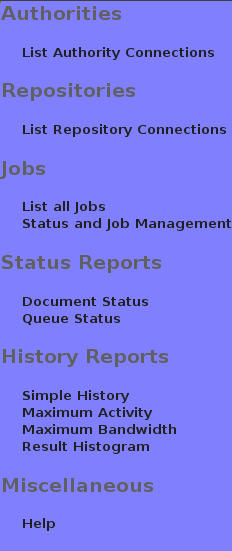
\includegraphics[width=80pt]{crawler-sidebar}}
\end{picture}


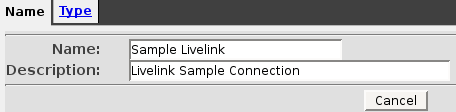
\includegraphics[width=300pt]{edit-authority-tab1}

This is the first tab of the tabbed interface you will use to edit
authority connections. The next tab is shown as follows:

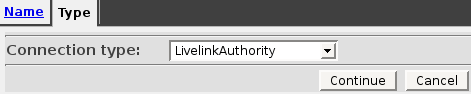
\includegraphics[width=300pt]{edit-authority-tab2}

In the first two tabs you must provide a name, description, and an
authority type. The name should be unique, as you will use it to
select this connection later when making repository connections. The
description should explain the authority connection to you or another
administrator. The authority type is the type of authority to which
you will connect.

Once you have filled in those tabs, click continue, and then 
you must fill in the following extra fields if you choose to
configure a Livelink authority connection:

% Licensed to the Apache Software Foundation (ASF) under one or more
% contributor license agreements. See the NOTICE file distributed with
% this work for additional information regarding copyright ownership.
% The ASF licenses this file to You under the Apache License, Version 2.0
% (the ``License''); you may not use this file except in compliance with
% the License. You may obtain a copy of the License at
%
% http://www.apache.org/licenses/LICENSE-2.0
%
% Unless required by applicable law or agreed to in writing, software
% distributed under the License is distributed on an ``AS IS'' BASIS,
% WITHOUT WARRANTIES OR CONDITIONS OF ANY KIND, either express or implied.
% See the License for the specific language governing permissions and
% limitations under the License.

\subsubsection{Configuring a Livelink Authority Connection}

The following options are specific to Livelink:

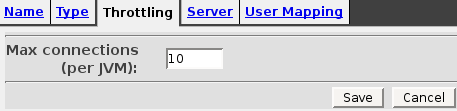
\includegraphics[width=300pt]{edit-authority-tab3}

\begin{itemize} 

\item \textbf{Max Connections (per JVM):} Here you can specify a
maximum number of connections for your authority
connection. \ifCombinedConnectorGuide The maximum number of
connections can affect system licensing and performance. See the Max
Connections item on page \pageref{max-auth} for more details.\fi

\ifLivelinkGuide
The maximum number of connections per JVM is important for two reasons.
First, the number of connections may impact the licensing on your document
server, depending on the repository. If you have a finite number of
Livelink connections available, they will be split between the authority
connector, which authorizes user access to documents, and the repository
connector, which actually downloads the documents to the appliance.

Second, the number of connections may impact the resources
available on the appliance. If the connector framework is slowing down
your appliance, lowering this number should help.
\fi

\end{itemize}

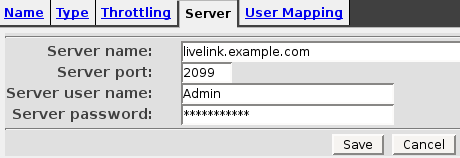
\includegraphics[width=300pt]{edit-authority-tab4}

\begin{itemize}

\item \textbf{Server name:} The name of the Livelink server from which
you wish to get authorization information.

\item \textbf{Server port:} The port on the Livelink server to which you
should connect. If you don't know what value this should be, ask your
Livelink administrator.

\item \textbf{Server user name:} The username you were given by your
Livelink administrator for connecting to the server. (The user account
must have sufficient authority to retrieve file ACLs.)

\item \textbf{Server password:} The password you were given by your
Livelink administrator for the above username.

\end{itemize}

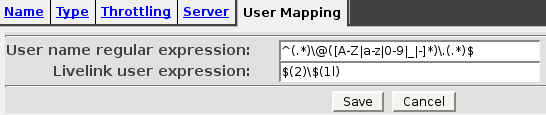
\includegraphics[width=300pt]{edit-authority-tab5}

\begin{itemize}

\label{regex}
\item \textbf{User name regular expression:} In many cases, the username
that an end-user will authenticate to GTS with is not the same as the
username that the Livelink server expects. This regular expression is used
to break the incoming username into pieces that can then be processed by
the next regular expression to produce a proper Livelink user name. The
default regular expression, \\ \verb+(.*)\@([A-Z|a-z|0-9|_|-]*)\.(.*)+,
separates an Active Directory \\ username of the form USER@DOMAIN.COM
into three distinct portions: USER, DOMAIN, and COM. In many cases,
this expression will be sufficient for you.

\note{If you are not familiar with regular expressions, there
are a variety of tutorials available on the web, including
\url{http://gnosis.cx/publish/programming/regular_expressions.html}
and \url{http://perldoc.perl.org/perlrequick.html}. If you still have
difficulty with these settings, please contact Customer Support (see
page \pageref{SupportContact}).}

\item \textbf{Livelink user expression:} Once you have deconstructed
the Active Directory username, you need to put it back together as an
appropriate Livelink username for your site's Livelink instance. The
default is the expression \verb+$(2)\$(1l)+, which takes the second value
from the first regular expression (DOMAIN), adds a backslash
(\verb+\+), and then puts the first value from the first expression in
place in lowercase (user), producing \verb+DOMAIN\user+. Depending on
how your Livelink instance is configured, you may need to change this
value. 

This expression may contain either plain text or variable expressions
such as \verb+$(2)+ above.  A variable expression, which must be of
the form \verb+$(N)+ where N is a number, represents a string from the
regular expression defined previously. You can force the string to be
all uppercase or lowercase by appending a \verb+u+ or \verb+l+ to the
string number. For example, to make the third string all in uppercase,
you would use \verb+$(3u)+. A dollar sign character must be escaped
with another dollar sign before it, so \verb+$$+ in this text box will
produce \verb+$+ in the user expression.

\end{itemize}

After entering this information, you will be taken to the authority
connection status page for this authority:

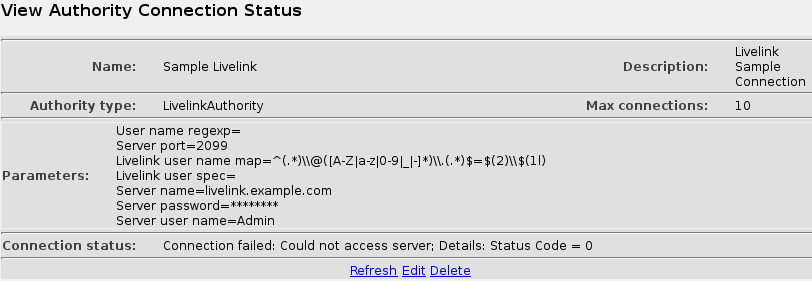
\includegraphics[width=300pt]{view-auth-conn-status}

In this example (which does not contain accurate information for any
Livelink server), the Connection Status is ``Connection failed.''
If you see this message, you most likely have incorrectly entered one
of the fields, and should click ``Edit'' to fix the data. If you have
entered everything as you intended, please inform your Livelink administrator;
you may not have been given the correct information.



\subsection{Creating Repository Connections}

Once you have created an authority connection, you need to create a
repository connection.
To do so, click ``List Repository Connections'' on the sidebar menu. Then,
when presented with the list of repository connections, click ``Add a
new connection.'' You will see the following two tabs:

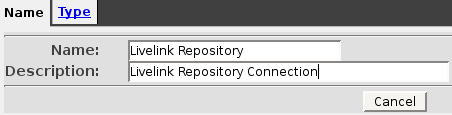
\includegraphics[width=300pt]{edit-repository-tab1}

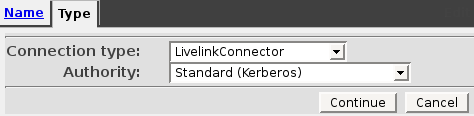
\includegraphics[width=300pt]{edit-repository-tab2}

Now you must provide a name, description, connector type, and
authority type for your new repository connection. The name should be
unique, as you will use it to select this connection later when
defining jobs. The description should explain the repository
connection to you or another administrator.  The connector type is the
type of repository from which you will get documents, in this case a
LivelinkConnector. The authority type is the type of authority from
which you will get authorization information. Typically, you will
select the Livelink authority connection that you have set up to
associate with this server; the permissions associated with the
ingested documents will be the same as the permissions of the original
documents in the Livelink repository. If you intend to force AD ACLs
on your documents (see page \pageref{ForceACL}), then you should
select ``Standard (Kerberos)'' here.


Once you have filled in those tabs, click continue to move on to the
repository-specific options.

% Licensed to the Apache Software Foundation (ASF) under one or more
% contributor license agreements. See the NOTICE file distributed with
% this work for additional information regarding copyright ownership.
% The ASF licenses this file to You under the Apache License, Version 2.0
% (the ``License''); you may not use this file except in compliance with
% the License. You may obtain a copy of the License at
%
% http://www.apache.org/licenses/LICENSE-2.0
%
% Unless required by applicable law or agreed to in writing, software
% distributed under the License is distributed on an ``AS IS'' BASIS,
% WITHOUT WARRANTIES OR CONDITIONS OF ANY KIND, either express or implied.
% See the License for the specific language governing permissions and
% limitations under the License.

\subsubsection{Configuring a Livelink Repository}

You must fill in the following extra tabs if you are creating a
Livelink repository connection:

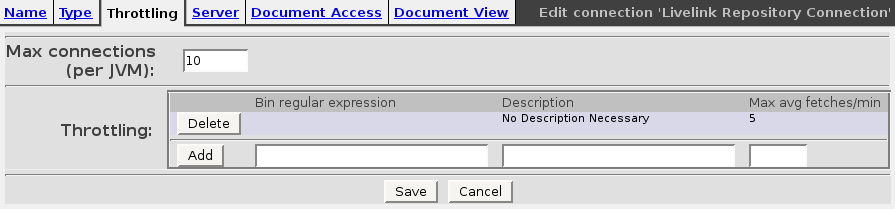
\includegraphics[width=300pt]{edit-repository-tab3}

\begin{itemize}

\item \textbf{Max connections (per JVM):} Here you can specify a
maximum number of connections for your repository. \ifCombinedConnectorGuide
The maximum number of connections per JVM is important for three
reasons; licensing, appliance resources, and the possiblity of
overwhelming the ingestion interface. For a more complete explanation,
see the Max Connections item on page \pageref{maxrepocon}.\fi

\ifLivelinkGuide
The maximum number of connections per JVM is important for three reasons.
First, the number of connections may impact the licensing on your document
server, depending on the repository. If you have a finite number of
Livelink connections available, they will be split between the authority
connector, which authorizes user access to documents, and the repository
connector, which actually downloads the documents to the appliance.

Second, the number of connections may impact the resources
available on the appliance. If the connector framework is slowing down
your appliance, lowering this number should help.

Third, only ten document streams can be processed by the appliance
at one time.  If you are also using other repository connectors or
the \command{ingest} command on the appliance, you should reduce this
number to prevent contention for the Ingestion interface. The Livelink
Connector will never overwhelm the interface on its own, but when other
applications are also using the ingestion interface, it may be best to
set the number of repository connections to five or even fewer.
\fi

\item \textbf{Throttling:} This allows you to set a maximum document
fetch rate from the repository.


The maximum fetch rate allows you to set three things: Expression,
description, and fetches per minute. Expression allows you to provide
a regular expression to match against document bins.  Each document
ingested through a connector is associated with one or more document
bins. These bins represent the servers that the connector interacts
with to obtain the document.  Typically, a document will be associated
with only one document bin, representing the repository server hosting
the document. For some repository connections, documents ingested
through the connector can be hosted by different servers. In the
Livelink Connector, documents only come from one server, which you
will set on the following tab. Simply leave the expression blank; this
will match any server you enter on the following tab.  All you need to
set is the number of document fetches per minute.  Description is an
optional field that allows you to provide a short text description of
the throttle.  Once you have set the fetch rate and optional
description, click Add.


\end{itemize}

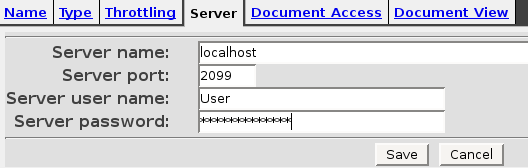
\includegraphics[width=300pt]{edit-repository-tab4}

\begin{itemize}

\item \textbf{Server name:} The name of the Livelink server from which you wish
to crawl documents.

\item \textbf{Server port:} The port on the Livelink server to which you
should connect. If you don't know what value this should be, ask your
Livelink administrator.

\item \textbf{Server user name:} The username you were given by your
Livelink administrator for connecting to the server. (The user account
must have sufficient authority to retrieve documents.)

\item \textbf{Server password:} The password you were given by your
Livelink administrator for the above username.

\end{itemize}

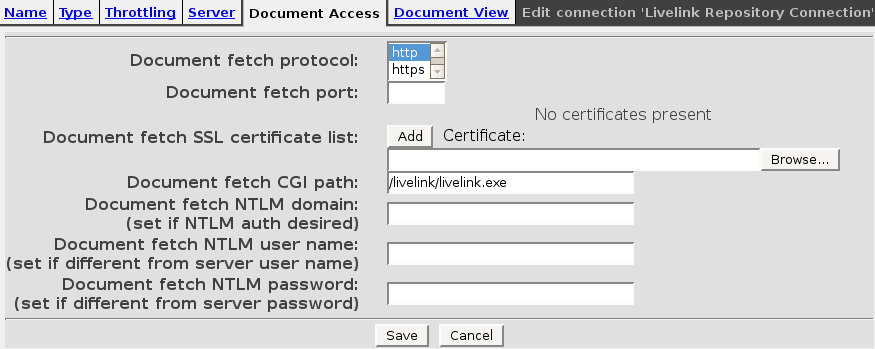
\includegraphics[width=300pt]{edit-repository-tab5}

These options all concern ``fetching'' documents, that is, the paths
that the Connector Framework should use when collecting documents for
ingestion to the MetaCarta search system. 

\begin{itemize}

\item \textbf{Document fetch protocol:} If you are connecting to an
open Livelink repository, choose ``http.'' If you are connecting using
SSL, choose ``https.''

\item \textbf{Document fetch port:} The port to use when connecting
to the Livelink server. If you are using the default port (80 for
http, 443 for https) you can leave this field blank. 

\item \textbf{Document fetch SSL certificate list:} Some Livelink servers
require that you authenticate via SSL before downloading documents. By
clicking the ``Browse'' button, you can select an SSL certificate that
the appliance should trust for authentication to the Livelink server. Clicking
``Add'' will upload the certificate to the appliance.

To get such a certificate, visit the Livelink repository from your
web browser and save the file, or ask your Livelink administrator.
For maximum robustness, you should add the certificate for the certificate
authority that signed the Livelink repository certificate rather than
the Livelink certificate itself. To do this, contact your site's security
administrators. In some cases, you may need more than one certificate.

\item \textbf{Document fetch CGI path:} The path on the Livelink server that the
appliance should use to crawl for documents.

\item \textbf{Document fetch NTLM domain:} The NTLM domain 
through which the crawler should access the Livelink repository, if required.

\item \textbf{Document fetch NTLM user name:} The user name to use for 
NTLM, if different from the user name used to connect to the server.

\item \textbf{Document fetch NTLM password:} The password to use for
NTLM, if different from the password used to connect to the server.

\end{itemize}

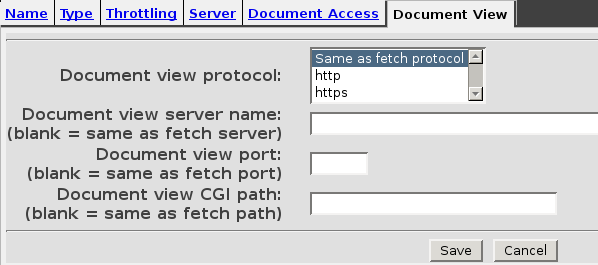
\includegraphics[width=300pt]{edit-repository-tab6}

These options all concern ``viewing'' documents, that is, the URLs
at which users are directed to documents when they see the documents
as search results. These options can be used to change the URLs of
documents crawled through Livelink before they are sent to the MetaCarta
Ingestion API. They do not change anything about the documents in the
Livelink repository itself. 

\begin{itemize}

\item \textbf{Document view protocol:} If end users are connecting to an open
Livelink repository, choose ``http.'' If users are connecting using SSL,
choose ``https.'' If users are connecting to the same Livelink instance
as the crawler, choose ``Same as fetch protocol.''

\item \textbf{Document view server:} The server to use when giving end
users links to a Livelink server as part of search results. If you
are using the same server as for document fetch, you can leave this
field blank.

\item \textbf{Document view port:} The port to use when giving end users
links to the Livelink server as part of search results. If you are using
the same port as for document fetch, you can leave this field blank.

\item \textbf{Document view CGI path:} The path on the Livelink server
that the end user should use when viewing document search results. This
is usually the same as the fetch path, but if it is not, you can set
it here. If this is different from the document fetch CGI path, it is
likely because the appliance has different permissions from normal users,
but it may also be because you want users to access a different Livelink
server from the appliance. This setting (along with the NTLM domain,
described above) determines the URL given to users of the Web Search
Interface, MetaCarta Search APIs, and the ESRI ArcMap Extension.

\end{itemize}


After entering this information, you will be taken to the repository 
connection status page for this repository:

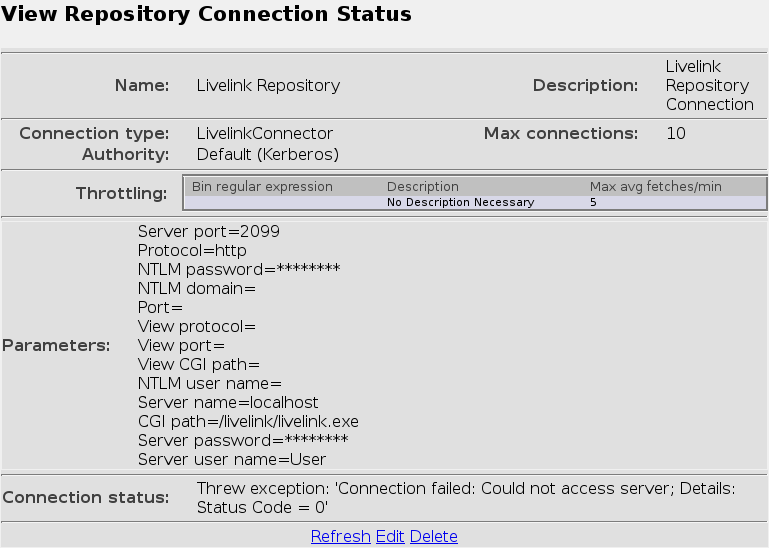
\includegraphics[width=300pt]{view-repo-conn-status}

In this example (which does not contain accurate information for any
Livelink server), the Connection Status is ``Connection failed.''
If you see this message, you most likely have incorrectly entered one
of the fields, and should click ``Edit'' to fix the data. If you have
entered everything as you intended, please inform your Livelink administrator;
you may not have been given the correct information.


\subsection{Creating and Running Jobs}

To run a job, click ``Status and Job Management'' on the sidebar menu.
You can run or edit existing jobs from this menu.

To create a new job, click ``List All Jobs'' on the sidebar menu. Then, when
presented with the list of current jobs, click ``Add a new job.'' You
will be presented with two tabs, in which you must fill in the following
information:

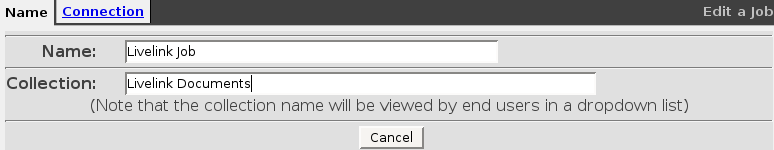
\includegraphics[width=300pt]{edit-job-tab1}

\begin{itemize}

\item \textbf{Name:} The name of the job. You will use this to identify
the job later.

\item \textbf{Collection:} The collection name metadata for all documents
in this job. End users can use this
name to select the set of documents in this job. For more information
on collection name metadata, please see the \documentref{MetaCarta
GTS Administrator's Guide}.

\end{itemize}

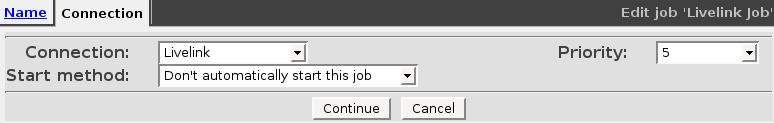
\includegraphics[width=300pt]{edit-job-tab2}


\begin{itemize}

\item \textbf{Connection:} The name of the repository connection you
wish to use for this job. You select this from the list of repository
connections you have already made. You may have more than one job use
the same repository connection, but if you have two jobs crawl the same
documents, the documents will have the metadata and collection name
associated with whatever job crawled the document most recently. This
will cause unpredictable results when searching those collections,
searching for those documents, or trying to delete those collections.
We recommend never crawling the same document in two different jobs.

\item \textbf{Start method:} Whether you want to start this job the next
time jobs are scheduled to run (``Start when schedule window starts''),
immediately after you finish defining it (``Start even inside a schedule
window''), or not at all (``Don't automatically start this job'').

\item \textbf{Priority:} From 1 (highest) to 10 (lowest), the priority
this crawl should have if it must compete for resources with other
crawls on the appliance. You should not need to change this unless you
are running more than one crawl at the same time; if you are, assign a
higher priority to the crawls whose documents you want to be processed
preferentially before documents from other jobs.

\end{itemize}

After filling in those options, click ``Continue,'' and you will be
presented with five additional repository-specific tabs. 

% Licensed to the Apache Software Foundation (ASF) under one or more
% contributor license agreements. See the NOTICE file distributed with
% this work for additional information regarding copyright ownership.
% The ASF licenses this file to You under the Apache License, Version 2.0
% (the ``License''); you may not use this file except in compliance with
% the License. You may obtain a copy of the License at
%
% http://www.apache.org/licenses/LICENSE-2.0
%
% Unless required by applicable law or agreed to in writing, software
% distributed under the License is distributed on an ``AS IS'' BASIS,
% WITHOUT WARRANTIES OR CONDITIONS OF ANY KIND, either express or implied.
% See the License for the specific language governing permissions and
% limitations under the License.

\subsubsection{Livelink Job Options}

In the Livelink-specific tabs, you will have the following additional
settings:

\bigimage{edit-job-tab3}

\ifLivelinkGuide
% Licensed to the Apache Software Foundation (ASF) under one or more
% contributor license agreements. See the NOTICE file distributed with
% this work for additional information regarding copyright ownership.
% The ASF licenses this file to You under the Apache License, Version 2.0
% (the ``License''); you may not use this file except in compliance with
% the License. You may obtain a copy of the License at
%
% http://www.apache.org/licenses/LICENSE-2.0
%
% Unless required by applicable law or agreed to in writing, software
% distributed under the License is distributed on an ``AS IS'' BASIS,
% WITHOUT WARRANTIES OR CONDITIONS OF ANY KIND, either express or implied.
% See the License for the specific language governing permissions and
% limitations under the License.

\begin{itemize}
\label{scheduling}

\item \textbf{Schedule type:} Whether you want to scan every document
once or dynamically recrawl content in your repository. 

When scanning every document once, the crawler marks all documents that
have been previously crawled in this job as potentially to be deleted,
adds all seed documents to its queue and marks them as pending, processes
pending documents, marking them completed as they are ingested, and then
deleted all of the documents that were not recrawled. A document might
not be recrawled because it no longer exists, or the job specification
might have been changed to no longer include the document.

When dynamically recrawling documents, the crawler does not start by
marking all documents as potentially deletable; instead, it begins with
all of the seed documents, and continues adding to its list, periodically
re-adding the initial seed documents. If a document is removed from the
source, it will expire in the expiration interval (see below).

\item \textbf{Expiration Interval (if continuous):} The length of the
interval (in minutes) that the appliance will retain a document
crawled by this job after the document no longer appears in the
repository. After this interval, the missing document will be removed
from the appliance's index and archive. Leave the expiration interval
blank to keep missing documents indexed in GTS.

\item \textbf{Recrawl interval:} If you are dynamically recrawling
documents, how long, in minutes, the crawler should wait before
crawling documents a second time.

\item \textbf{Reseed interval:} If you are dynamically recrawling
documents, how long, in minutes, the crawler should wait before
looking for new documents to crawl. \ifMeridioGuide This connector
identifies all documents for ingestion through seeding; if the reseed
interval is infinite, the job will not ingest documents placed in the
repository during run time. (The job automatically reseeds whenever it
is started.) The default interval of 60 minutes is an appropriate
reseed rate. \fi \ifFilenetGuide This connector identifies documents
for ingestion during seeding. If you change the document inclusion
criteria, reseeding is required to identify new documents. Similarly,
documents placed in the repository while the job is running will not
be identified until the crawl is reseeded.  (The job automatically
reseeds whenever it is started.) The default interval of 60 minutes is
an appropriate reseed rate. \fi

\item \textbf{Scheduled time:} Allows you to define a time you wish
the job to run using a series of selection boxes. The first box refers
to the day of the week you wish the job to run, with an option to have
the job run any day of the week. The second box allows you to select
the start hour, with an option to start the job at any hour. The third
box allows you to specify which minute after the hour that you wish
the job to start. The fourth box allows you to specify what months of
the year you wish the job to run, with an option for the job to run
any month. The last box allows you to specify the day of the month you
wish the job to start, including any day of month.


You can scroll through each of the five boxes in this setting using
the arrow keys on your keyboard or by using the scroll bar on the
right side of the box.  If you want to select more than one value,
hold down control as you scroll and click the values that you want to
select. This allows you to define multiple windows with the same
length, for example by selecting Monday, Wednesday, and Friday at the
same time.

\item \textbf{Maximum run time:} The longest you will allow the job to
run, in minutes. For example, if you want to start a job at 2 AM but
force it to stop at 8 AM so that users have access to the repository,
you should set this value to 360 minutes. If the job is not complete by the
end time, documents that have already been found will be indexed, and
the rest of the crawl will continue at the beginning of the next
schedule interval. 

When you have defined the scheduled time and assigned a maximum run
time, click on the ``Add Scheduled Time'' button. A new schedule box
will appear below the scheduled time, allowing you to create
additional scheduled run times.

Here is a sample schedule for a job that will run every
Monday from 2 am to 6 am:

\begin{changemargin}{-.3in}{0in} 
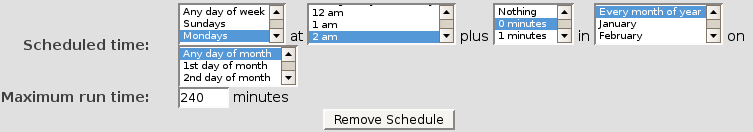
\includegraphics[width=300pt]{sample-schedule}
\end{changemargin}

If you do not have at least one scheduled time, the job will
only run when run manually (see page \pageref{ManageJobs}), and will
not automatically update the index on the appliance based on changes
to the repository.

You can remove a scheduled time by clicking the ``Remove Schedule''
button.

\end{itemize}

\fi

\ifCombinedConnectorGuide
This tab presents scheduling options. Here you can generate one or
more scheduled run times for the job. For a complete description of
the scheduling options, see the description starting on page
\pageref{scheduling}.
\fi

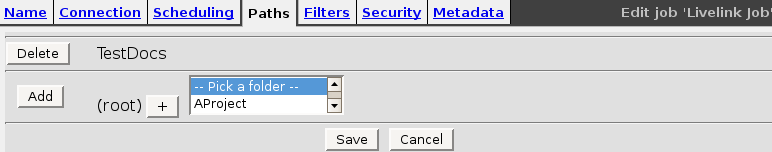
\includegraphics[width=300pt]{edit-job-tab4}

\begin{itemize}

\item \textbf{Roots:} The base directories in Livelink from which you
want your crawl to start. You may select zero, one, or more than one
(though if you select zero, your appliance will not crawl anything). 
To select a directory, select the directory name, click the ``+''
button, and then click ``Add.'' The directory will appear inside the selection
box; you can click the ``Delete'' button next to it to remove it from
your list of directories to be crawled.

\end{itemize}

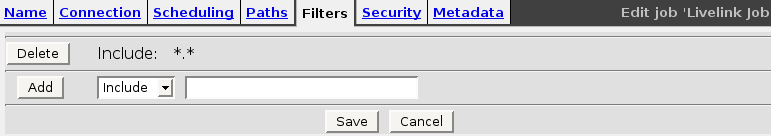
\includegraphics[width=300pt]{edit-job-tab5}

\begin{itemize}

\item \textbf{Filters:} You must define the files that will be 
crawled and indexed during this job. You do this by specifying filetypes
of the form ``\*.XYZ.'' You must specify at least one filetype to 
include, or you will not crawl any documents.

For example, if you want to crawl .QZX
files, you can enter ``\*.QZX'', select ``Include'', and then click Add.
You may define multiple inclusions and exclusions; if an exclusion and an
inclusion conflict, the first one you entered is followed.  

% Licensed to the Apache Software Foundation (ASF) under one or more
% contributor license agreements. See the NOTICE file distributed with
% this work for additional information regarding copyright ownership.
% The ASF licenses this file to You under the Apache License, Version 2.0
% (the ``License''); you may not use this file except in compliance with
% the License. You may obtain a copy of the License at
%
% http://www.apache.org/licenses/LICENSE-2.0
%
% Unless required by applicable law or agreed to in writing, software
% distributed under the License is distributed on an ``AS IS'' BASIS,
% WITHOUT WARRANTIES OR CONDITIONS OF ANY KIND, either express or implied.
% See the License for the specific language governing permissions and
% limitations under the License.

MetaCarta GTS currently supports the following filetypes:

\begin{itemize}
\item ASCII Text Files with or without extensions (.txt, etc...)
\item HTML Documents (.htm, .html)
\item Adobe\circler\ Acrobat\circler\ files (.pdf)
\item Adobe PostScript\circler\ files (.ps)
\item Microsoft\circler\ Word\circler\ documents (.doc)
\item Microsoft Excel\circler\ spreadsheets (.xls)
\item Microsoft PowerPoint\circler\ presentations (.ppt)
\item Rich Text Format documents (.rtf)
\end{itemize}

\note{Documents larger than 50MB are converted to plaintext and then truncated to 50MB.} 



To crawl and index all files, enter ``\*.\*'' and click Add.

\end{itemize}

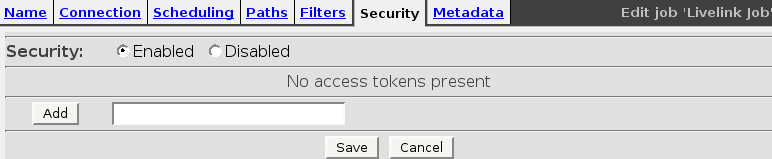
\includegraphics[width=300pt]{edit-job-tab6}

\begin{itemize}

\item \textbf{Security:} Allows you to control whether or not file ACLs,
or access control lists, are passed to the appliance with the files. If
you select ``Disabled'' here, all files crawled from Livelink will be
visible to all GTS users.

\item \ifLivelinkGuide \label{ForceACL}\fi \textbf{Access Tokens:} If you want to pass on
your own Active Directory ACLs instead of those used by Livelink---or
your Livelink instance does not contain Livelink ACLs---you can enter
them here.  You should enter one or more SIDs that you want to have
read permissions on the files crawled in this job. Two special
Livelink tokens can also be entered. The token ``SYSTEM'' represents
Livelink system administrators, while the token ``GUEST'' represents
users logged into Livelink as guests. For more information about AD
ACLs and SIDs, please see the security sections of the
\documentref{MetaCarta Appliance Administrator's Guide}.

\note{If you have disabled security, these ACLs will not be passed to
the appliance.}

\end{itemize}

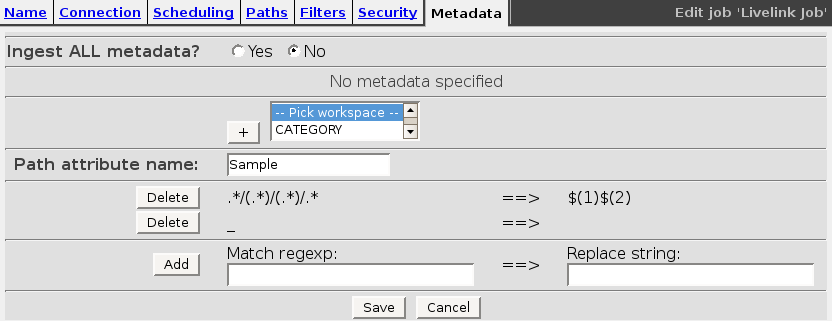
\includegraphics[width=300pt]{edit-job-tab7}

\begin{itemize}

\item \textbf{Ingest ALL metadata:} Choose yes if you want to ingest all 
metadata for each document crawled.

\item \textbf{Metadata:} The Livelink server stores various metadata
information about documents in its index.  You can select those metadata
fields here and have them sent along with the files you index as metadata.
Metadata will not be geographically parsed or used to create the index
on the MetaCarta appliance; however, with the SOAP Search API, you
can construct searches based specifically on this metadata. For more
information on the SOAP Search API, please see the \documentref{MetaCarta
SOAP Search API Guide}.

\item \textbf{Path attribute name:} The name of the GTS metadata
attribute to which you want to attach Livelink file path data, if any.

\item \textbf{Path-value mapping:} The regular expressions
and substitutions that you want to use to collect information
from the Livelink file path. Using the regular expression
rules on page \pageref{regex}, you can construct one or more
expressions. In the example shown, there are two expressions. The
first, \verb+.*/(.*)/(.*)/.*+ to \verb+$(1) $(2)+, would change the
directory path ``Project/Folder\_1/Folder\_2/ Filename'' into ``Folder\_1
Folder\_2.'' The second, \_ to a space, would then be applied to turn
the metadata into ``Folder 1 Folder 2.'' It is important to allow more
than one transform so that you can, if necessary, extract text data and
then parse the extracted data. The end result of the last transform will
be ingested as the value of the metadata attribute defined previously.

\end{itemize}

After entering this information, you will be taken to the status page
for this job:

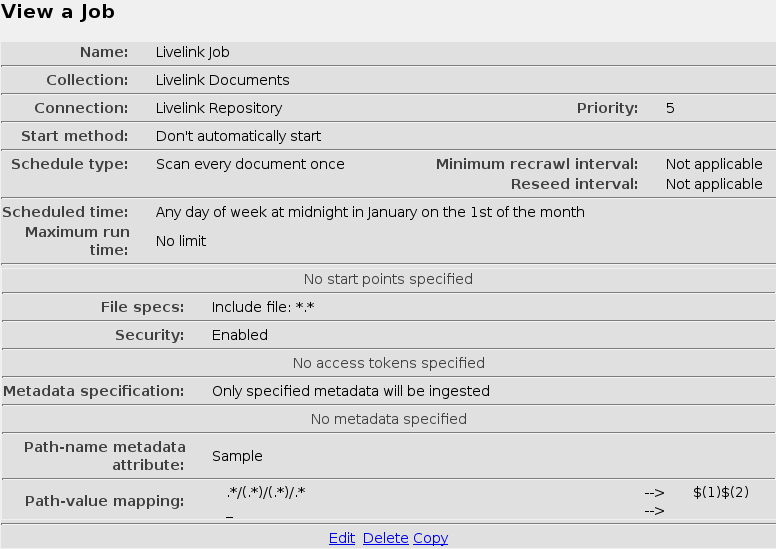
\includegraphics[width=300pt]{view-job-status}


\subsection{\label{ManageJobs}Status and Job Management}

You can then look at the status of your job by clicking ``Status and 
Job Management'' on the sidebar. You will see a list of one or more jobs
much like this one:

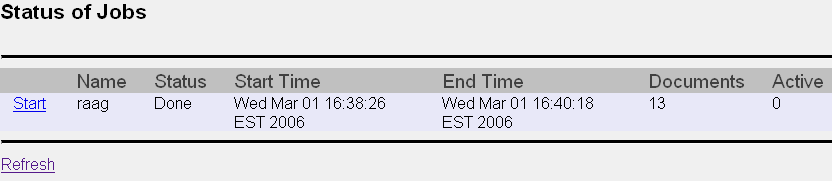
\includegraphics[width=300pt]{jobs-list}

You can start any crawl you like immediately from this interface by
clicking ``Start'' next to the name of the crawl. This interface also
allows you to see how many documents have been crawled; this information
may help you structure and plan future crawls.

\note{Refresh this page by clicking the ``Refresh'' link at the bottom
of the page, not by clicking your browser's reload button.}

\section{Reports}

The Livelink Connector interface can generate four types of reports:

\begin{itemize}

\item Simple History, which lets you list an ordered set of log events
based on chosen criteria

\item Maximum Activity, which lets you see the period of time in
which a certain event happened most often

\item Maximum Bandwith, which lets you see the period of time in
which the most bandwidth was used 

\item Result Histogram, which provides log information that would be
appropriate for constructing a histogram or other diagram

\end{itemize}

Each of these reports allows you to specify a connection, one or more
activities, a start time, an end time, an entity match, and a result code
match.  Some also allow you to specify an identifier class description
and a sliding window size. This section will show sample results for
each type of report and an explanation of the fields selected.

\subsection{Simple History}

This report was generated by selecting ``Sample Livelink Repository,'' 
clicking Continue, selecting ``fetch document,'' and clicking Go.

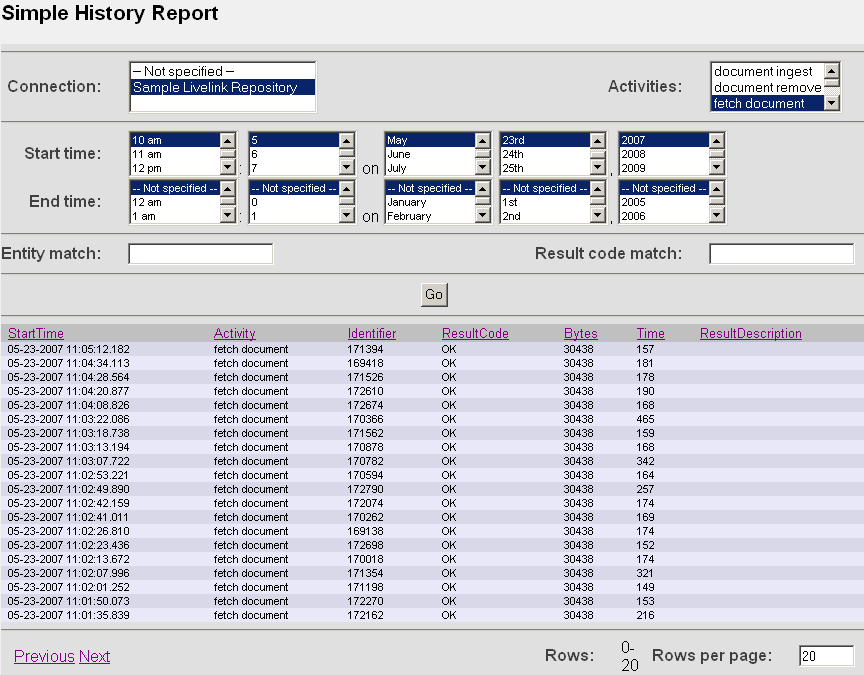
\includegraphics[width=300pt]{simple-history-report}

\begin{itemize}

\item \textbf{Connection:} The repository connection from which to generate
a report.

\item \textbf{Activities}: What crawler activities you would like to see. 
Your options are document ingest, document remove, fetch document, find 
documents, job abort, job continue, job end, job start, and job wait. 

\item \textbf{Start time}: The earliest time in the crawler logs to be
considered for this query.  Choose ``Not specified'' for any field to
start at the beginning of the crawler's logs.

\item \textbf{End time:} The latest time in the crawler logs to be
considered for this query. Choose ``Not specified'' for any field 
to end at the current time.

\item \textbf{Entity match:} A regular expression (see page
\pageref{regex}) to limit the Identifier field. If the entity match
field in the example above had been \texttt{\^{}17}, only document
fetches with Identifiers starting with 17 would be shown.

\item \textbf{Result code match:} A regular expression to limit the
ResultCode field.

\end{itemize}

You can sort the history report by any of the returned fields; to do so,
click the field names.


\subsection{Maximum Activity}

This report was generated by selecting ``Sample Livelink Repository,''
clicking Continue, selecting ``document ingest,'' changing the Identifier
class description, and clicking Go.

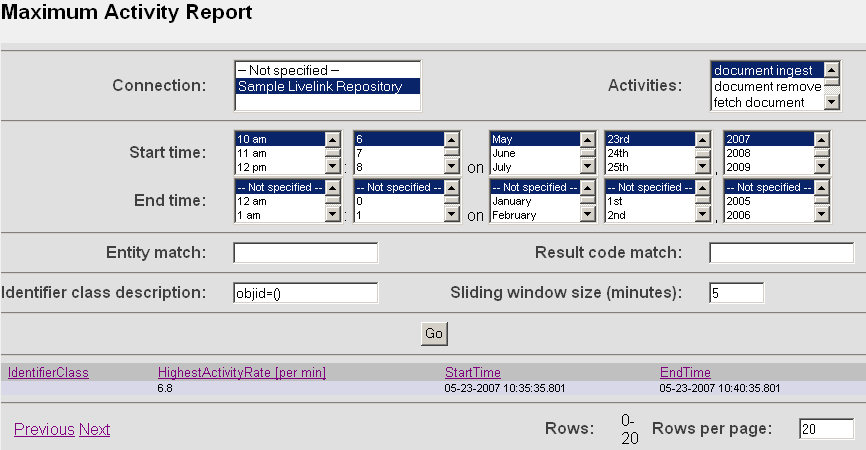
\includegraphics[width=300pt]{maximum-activity-report}

This form offers two more fields than the previous form:

\begin{itemize}

\item \textbf{Identifier class description:} A regular expression
that determines how to group identifiers together. If this were set to
\texttt{(.*)}, there would be no grouping, and so there would be only one
ingestion event per document. If this were set to \texttt{objid=(17)},
then all documents with identifiers beginning with 17 would be grouped
together. The setting in the example, \texttt{objid=()}, groups all
documents together. Some other possibilities:

\begin{itemize}

\item \texttt{1(.)}: (up to) Ten groups of documents whose identifier starts
with 1, labeled 0-9, grouped by the second digit of their identifier.

\item \texttt{()}: One group of documents containing all documents 
regardless of identifier.

\item \texttt{17}: One group of documents whose identifier contains
the string ``17.''

\item \texttt{\^{}17}: One group of documents whose identifier \emph{starts}
with the string ``17.''

\end{itemize}

\item \textbf{Sliding window size}: The search interval in minutes.

\end{itemize}

The report returned will have only one result per group with one or more
documents in it, if there is a clear highest activity rate, or a list of
all the results tied for highest activity rate if there are more than one.

\subsection{Maximum Bandwidth}

This report was generated by selecting ``Sample Livelink Repository,''
clicking Continue, selecting ``document ingest,'' changing the Identifier
class description, and clicking Go.

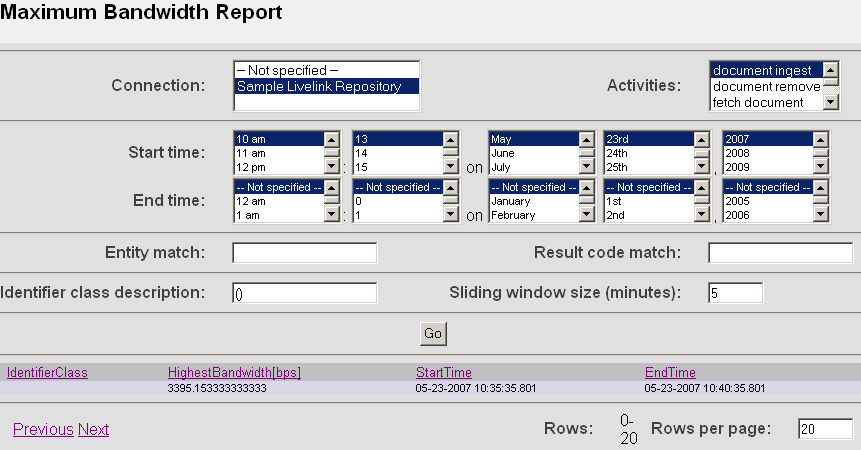
\includegraphics[width=300pt]{maximum-bandwidth-report}

This form offers the same fields as the maximum activity form, and
returns similar results; instead of tracking events per time window,
it tracks the window with the highest average bandwith usage, measured
in bytes per second. Again, the identifier class description has been
changed to a regular expression that will match all identifiers (and
thus in this case documents).

\subsection{Result Histogram}

This report was generated by selecting ``Sample Livelink Repository,''
clicking Continue, selecting ``document ingest,'' and clicking Go.

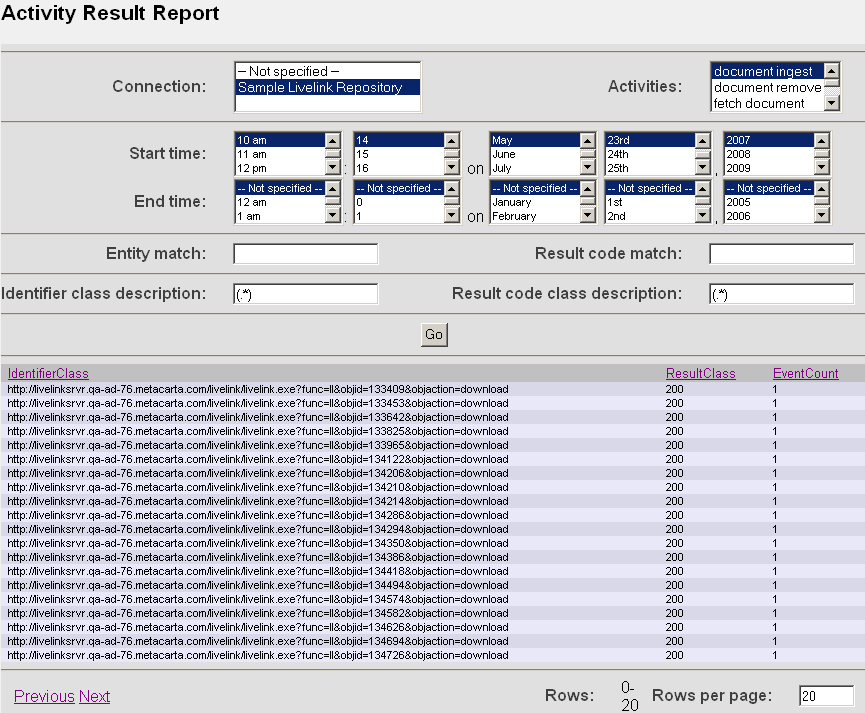
\includegraphics[width=300pt]{activity-result-report}

This form adds one new field:

\begin{itemize}

\item \textbf{Result code class description:} A regular expression that
determines how to group result classes together; like Identifier class
descriptions but for result classes.

\end{itemize}

This report does not produce an actual histogram, but provides data that
could be used to generate histograms.  

% This is a little sparse, but that's basically all this is, so.

\end{changemargin}
